\documentclass[14pt,a4paper]{article}
\usepackage{graphicx} 
\usepackage{hyperref}
\hypersetup{hidelinks}
\hypersetup{colorlinks=true}
\usepackage{CJKutf8}
\setlength\parindent{0pt} 
\begin{CJK}{UTF8}{gkai}

\renewcommand{\labelenumi}{\alph{enumi}.} 
\renewcommand\contentsname{目录}
\title{ \Huge 图像处理系统 \\\LARGE 总体设计}
\author{\newline \\\\\\ \textsc{\Large林悦如,刘涵宇,林宇翔}  } 
\date{\Large 2018-08-22} 

\begin{document}

\newpage
\maketitle 

\begin{center}
\begin{tabular}{l r l r}
\\ \\ \\ \\ 
\large 项目时间&: & 2018-07-12 - 2018-07-23 & \\ \\  
\large 项目参与人&: & \large3160104062 & \large \href{mailto:544766109@qq.com}{刘涵宇}\\
\large & &\large 3160102459 & \large\href{mailto:2106706074@qq.com}{林宇翔} \\
\large & &\large3140103548 &\large\href{mailto:lo0g1t7031@gmail.com}{林悦如(组长)} \\ \\
\large 指导人&: & \large浙江大学 & \large 袁昕 \\\\
\large 项目主页&: & \large \href{https://www.github.com/SummerCPP/segprototype/}{SummerCPP/segprototype/}
\end{tabular}
\end{center}


%===============================================
%		目录
%===============================================
\newpage
\hypersetup{colorlinks=false}
\tableofcontents



%===============================================
%		Chapter1 引言
%===============================================
\newpage
\section{引言}
\subsection{项目背景}
\subsubsection{系统名称}
图像处理系统
\subsubsection{任务提出者}
浙江大学科研和工程中的 C++训练课程任课老师-袁昕
\subsubsection{开发者 }
由浙江大学 2017-2018 学年短学期课程部分学生组成的项目组
\subsubsection{相关背景介绍}

为全面提高学生创新和实践能力,浙江大学科研和工程中的 C++训练课程分
为课堂教学和综合性实验两部分。综合性实验采取分组形式完成,每 3 个学生为
1 组,设有组长,通过让学生开发一个实际的 C++项目,深入了解科研和工程中
合作开发 C++项目基本原理、概念与方法,培养学生的应用开发能力与团队合作
精神。 锻炼学生综合运用每个环节所学知识解决。\\\\

图像处理是指对图像进行分析、加工、和处理,使其满足视觉、心理或其他要求的技术。图像处理是信号处理在图像领域上的一个应用。 图像处理领域的典型问题有几何变换,颜色处理,图像融合,降噪,边缘检测,分割,图像编辑,图像配准,图像增强,图像数字水印,图像压缩。\\

目前图像处理领域常用的软件开发工具有 OpenCV,ImageJ,Aphelion,
\\ Rapidminer等。这些开发库使得图像处理应用的开发变得十分方便。 


%===============================================
%		Chapter2 开发工具
%===============================================
\newpage
\section{开发工具}
\begin{itemize}
	\item Windows 10 
	\item Qt 5.10.0, Qt creator
	\item CMake 3.4.0
	\item Visual Studio 2017
\end{itemize}



%===============================================
%		Chapter 3 项目架构
%===============================================
\newpage
\section{项目架构}
\subsection{MVC框架}

\subsubsection{框架介绍}
MVC 全名是 Model View Controller,是模型(model)-视图(view)-控制器
(controller)的缩写,一种软件设计典范,用一种业务逻辑、数据、界面显示分离
的方法组织代码,将业务逻辑聚集到一个部件里面,在改进和个性化定制界面及
用户交互的同时,不需要重新编写业务逻辑。MVC 独特的发展起来被用于映射
传统的输入、处理和输出功能在一个逻辑的图形化用户界面的结构中。

\subsubsection{框架图示}
\nopagebreak
\begin{figure}[h]
\begin{center}
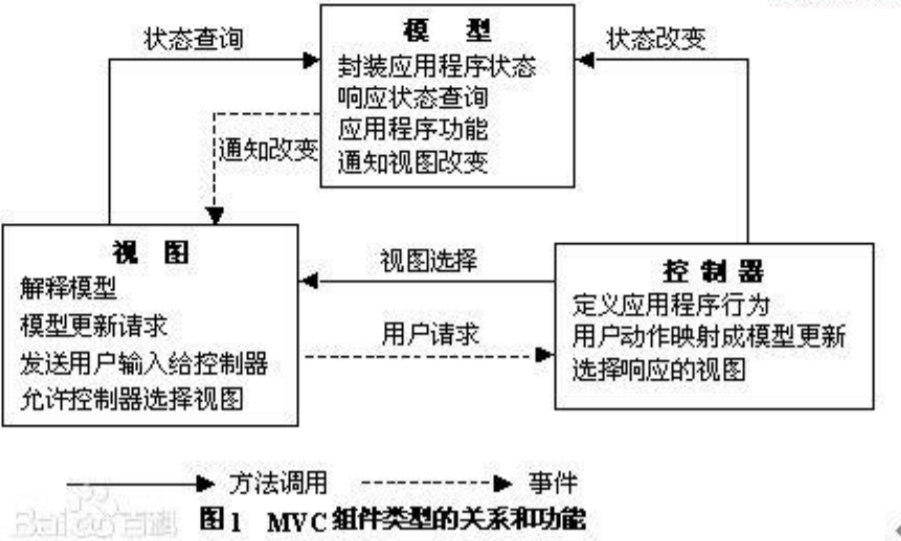
\includegraphics[width=0.8\textwidth]{image/mvc} % Include the image placeholder.png
\caption{MVC 模型示意图.}
\end{center}
\end{figure}

\subsubsection{框架内容}
MVC 指 MVC 模式的某种框架,它强制性的使应用程序的输入、处理和输出
分开。使用 MVC 应用程序被分成三个核心部件:模型、视图、控制器。它们各
自处理自己的任务。
\paragraph*{模型}
模型表示企业数据和业务规则。在 MVC 的三个部件中,模型拥有最多的处
理任务。例如它可能用像 EJBs 和 ColdFusion Components 这样的构件对
象来处理数据库,被模型返回的数据是中立的,就是说模型与数据格式无关,
这样一个模型能为多个视图提供数据,由于应用于模型的代码只需写一次就
可以被多个视图重用,所以减少了代码的重复性。
\paragraph*{视图}
视图是用户看到并与之交互的界面。对老式的 Web 应用程序来说,视图就
是由 HTML 元素组成
的界面,在新式的 Web 应用程序中,HTML 依旧在视
图中扮演着重要的角色,但一些新的技术已层出不穷,它们包括 Adobe Flash
和像 XHTML 等一些标识语言和 Web services。
\paragraph*{控制器}
控制器接受用户的输入并调用模型和视图去完成用户的需求,所以当单击
Web 页面中的超链接和发送 HTML 表单时,控制器本身不输出任何东西和
做任何处理。它只是接收请求并决定调用哪个模型构件去处理请求,然后再
确定用哪个视图来显示返回的数据。

\subsubsection{本项目中的框架实现}
\nopagebreak
本项目的原型系统采用MVC架构。\\\\
\begin{tabular}{ll}
视图: & QT 实现的基本 UI 界面 \\ 
控制器: & QT 实现的按钮,本身不做任何处理,\\
		   & 接收请求并决定调用哪个模型 \\
		    & 构件去处理请求,然后再确定用哪个视图来显示返回的数据。 \\
模型:		& 图像处理算法构件
\end{tabular}

\newpage
\subsection{MVVM框架}

\subsubsection{框架介绍}
MVVM是一种软件架构模式。MVVM有助于将图形用户界面的开发与业务逻辑或后端逻辑(数据模型)的开发分离开来,
这是通过GUI代码实现的。MVVM的视图模型是一个值转换器,这意味着视图模型负责从模型中暴露(转换)数据对象,以便轻松管理和呈现对象。视图模型处理大部分视图的显示逻辑。视图模型可以实现中介者模式,组织对视图所支持的用例集的后端逻辑的访问。
MVVM 中, 视图和试图模型之间采取了一种双向绑定(data binding)的方法,使得View的变动能够通过暴露出的数据属性自动反映在ViewModel上,反之亦然。

\subsubsection{框架图示}
\nopagebreak
\begin{figure}[h]
\begin{center}
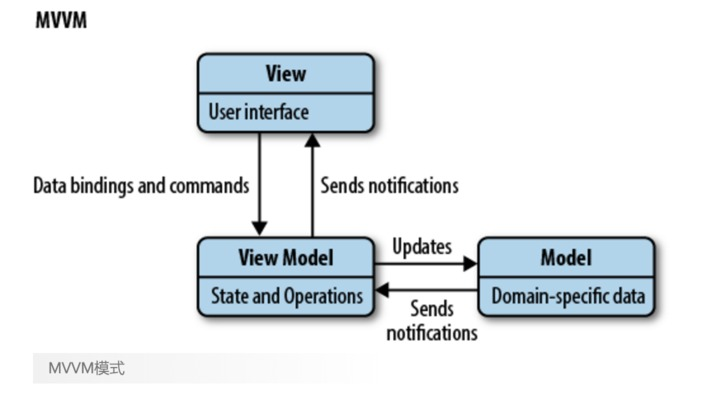
\includegraphics[width=0.9\textwidth]{image/mvvm} 
\caption{MVVM框架示意图.}
\end{center}
\end{figure}

\subsubsection{框架内容}

\paragraph*{视图}
视图是用户看到并与之交互的界面。视图负责界面和显示。它通过绑定ViewModel暴露的属性,和ViewModel进行数据绑定,不直接与Model交互。\\

\paragraph*{视图模型}
视图模型主要包括界面逻辑和模型数据封装,它是View和Model的桥梁,是对Model的抽象。

\paragraph*{数据模型}
Model与MVC模式一样,Model用于封装与应用程序的业务逻辑相关的数据以及对数据的处理方法。它具有对数据直接访问的权利,例如对数据库的访问,Model不依赖于View和ViewModel,也就是说,模型不关心会被如何显示或是如何被操作,模型也不能包含任何用户使用的与界面相关的逻辑。Model在实际开发中根据实际情况可以进行细分。

\subsubsection{本项目中的框架实现}
\nopagebreak
本项目后期采用MVVM架构。\\\\
\begin{center}
\begin{tabular}{ll}
视图: 	     & QT 实现的基本 UI 界面 \\ 
视图模型:   & 通过QT 的SIGNAL/SLOT/EVENT 机制,\\
				& 在被暴露的属性的Setter中\\
			    & 加上emit 语句,来通知视图相关属性的改变。\\
			    & 这不是实现双向绑定的好的方式,\\
			    & 因为这种实现方式严重依赖Qt,无法脱离Qt使用。\\
模型:		&负责维护系统的主要数据结构,调用算法层的业务逻辑。
\end{tabular}
\end{center}

%===============================================
%		Chapter 4 算法实现
%===============================================
\newpage
\section{算法实现}
\subsection{图像碎片化 Fragment}
\subsubsection{算法简介}

本算法可以将图片进行碎片化,达到一种较为艺术化的图片处理效果,在工作上可以为设计者带来一些灵感或帮助。
\subsection{高斯模糊 Gaussian}
\subsubsection{算法简介}
本算法可以将图片进行高斯模糊。是一种较为简易的图像处理算法。

\subsection{老旧照片 Old Movie}
\subsubsection{算法简介}
算法可以将图片做旧,实现一种老电影式的图片效果

\subsection{图片素描化 Sketch}
\subsubsection{算法简介}
算法可以将图片素描化,这是一种比较艺术化的处理效果
\subsubsection{算法效果}

\subsection{图片线条提取 Line}
\subsubsection{算法简介}
本算法可以提取图片的线条,为进一步设计打下基础



%===============================================
%		Chapter 6 协作情况
%===============================================
\newpage
\section{协作情况}
\subsection{GitHub 的使用}
\subsubsection{团队的创建 }
创建了我们的个人团队 SummerCPP,并邀请两位队友加入团队以便于对库进
行各种操作。
\nopagebreak
\begin{figure}[h]
\begin{center}
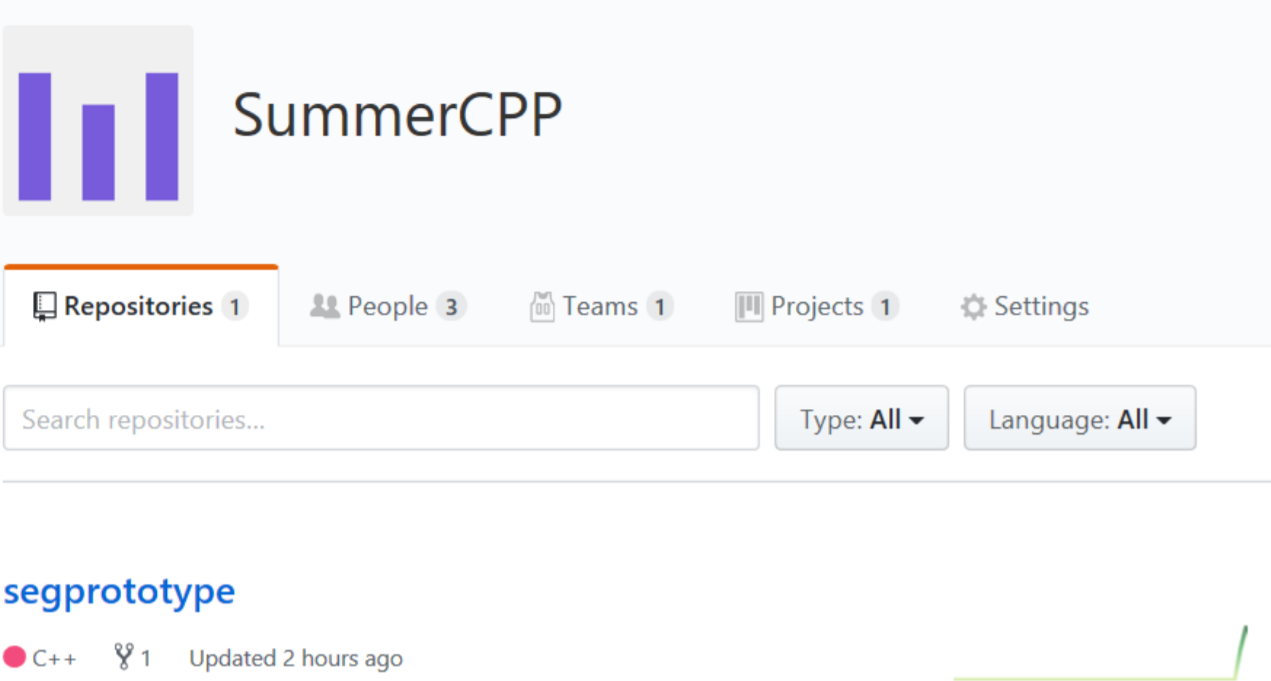
\includegraphics[width=0.8\textwidth]{image/team} 
\caption{团队界面.}
\end{center}
\end{figure}

\subsubsection{公有库的创建}
创建公有库 segprototype,团队成员在公有库上存放对工程做的更新与修改
\nopagebreak
\begin{figure}[h]
\begin{center}
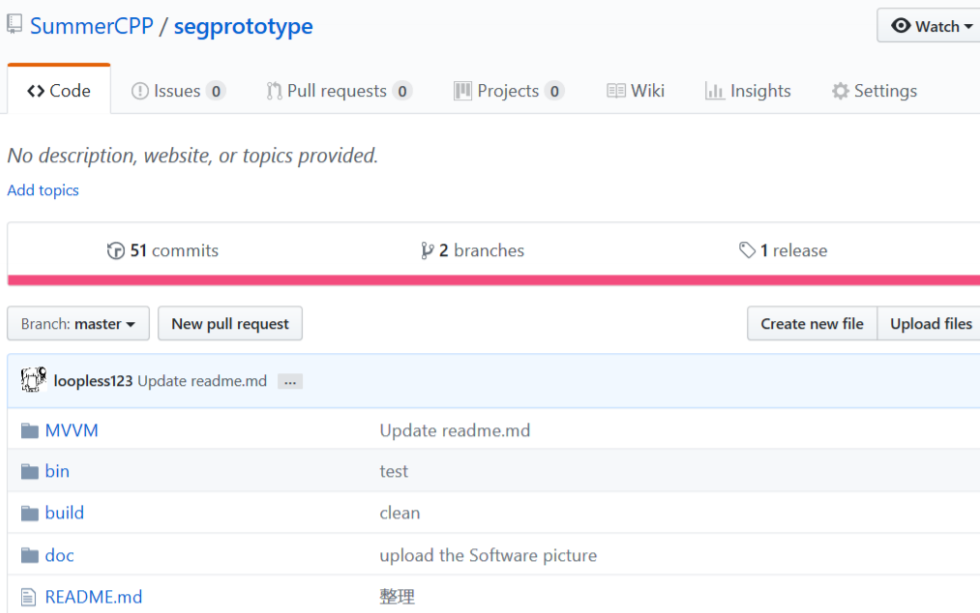
\includegraphics[width=0.8\textwidth]{image/seg} 
\caption{共有库界面.}
\end{center}
\end{figure}

\newpage
\subsubsection{工程的上传/更新/拉取/修改}
本团队使用 git 对库进行一系列的操作
\nopagebreak
\begin{figure}[h]
\nopagebreak
\begin{center}
\nopagebreak
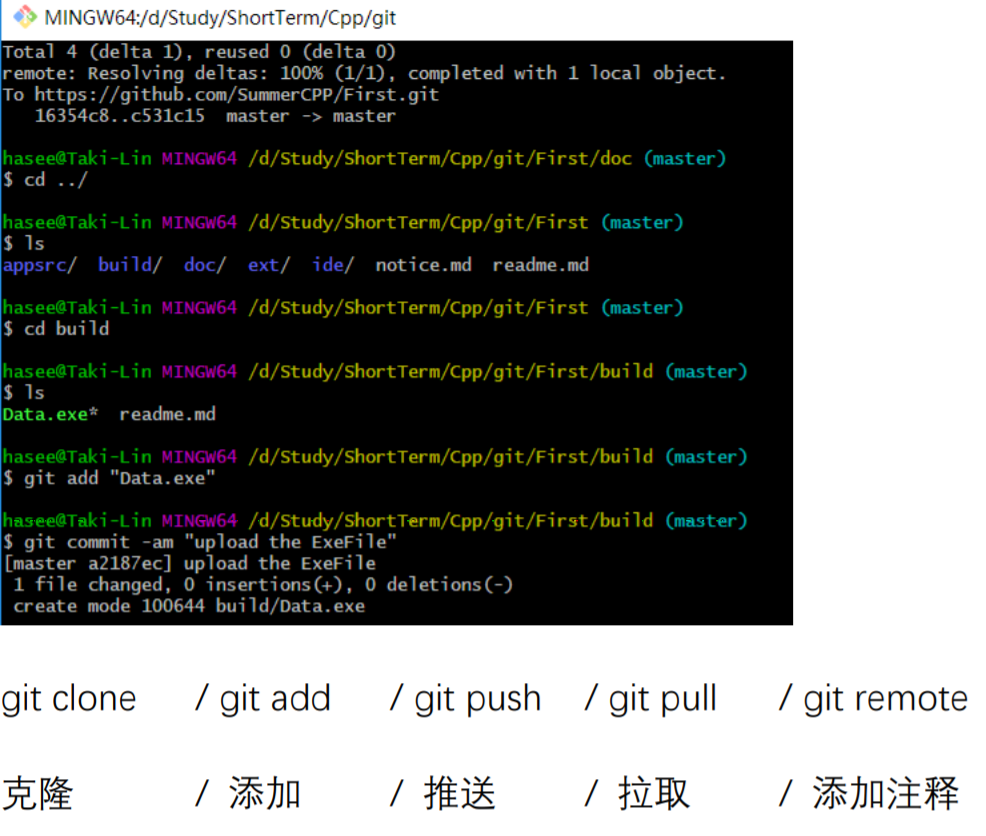
\includegraphics[width=0.8\textwidth]{image/term} 
\caption{Git Bash界面.}
\end{center}
\end{figure}

\subsection{团队工作流程}
\subsubsection{角色分工}
\nopagebreak
\begin{figure}[h]
\begin{center}
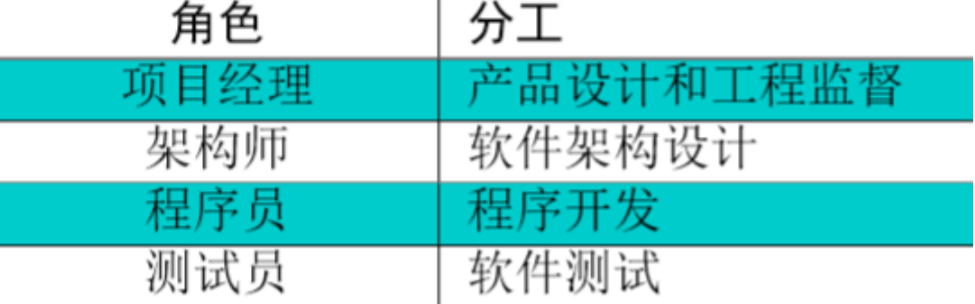
\includegraphics[width=0.8\textwidth]{image/role} 
\caption{团队角色.}
\end{center}
\end{figure}

\newpage
\subsubsection{开发流程}
本次项目分多个迭代轮次,每一轮各小组组员分别担任不同的角色对项目进
行开发。

\paragraph{第一轮迭代}
在第一轮迭代中,我们搭建了基本的开发环境,统一了开发工具的版本。开发了项目的原型系统。\\\\
\begin{figure}[h]
\begin{center}
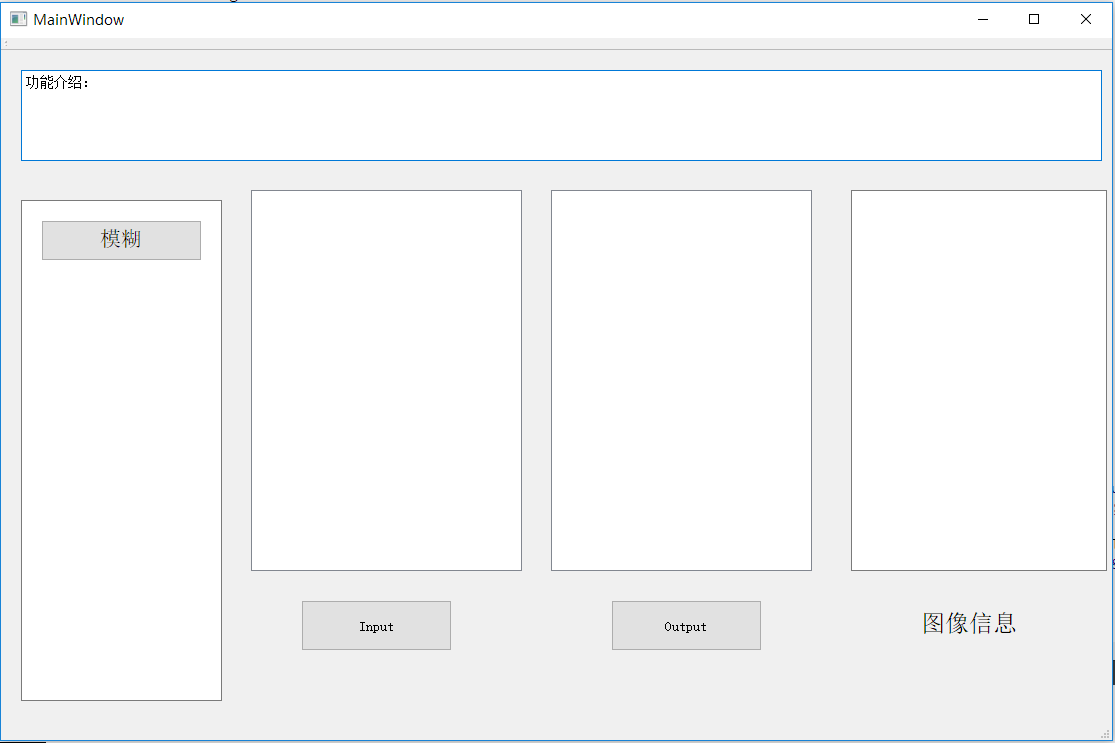
\includegraphics[height=0.4\textwidth]{image/prototype} 
\caption{系统原型.}
\end{center}
\end{figure}

这个阶段的分工情况如下所示:\\\\
\begin{center}
\begin{tabular}{lr}
	图形界面开发  &林宇豪 \\  
	算法层开发 &刘涵宇 \\
	模型开发,集成与测试&林悦如 \\
\end{tabular}
\end{center}

\newpage
\paragraph*{第二轮迭代}
第二轮迭代中,我们根据MVVM框架的结构重构了项目代码。同时重新设计了图形界面,并将其确定为最终的图形界面。 在原有系统的基础上,添加了新的功能。\\ 
项目代码结构如图7所示。 \\
\begin{figure}[h]
\begin{center}
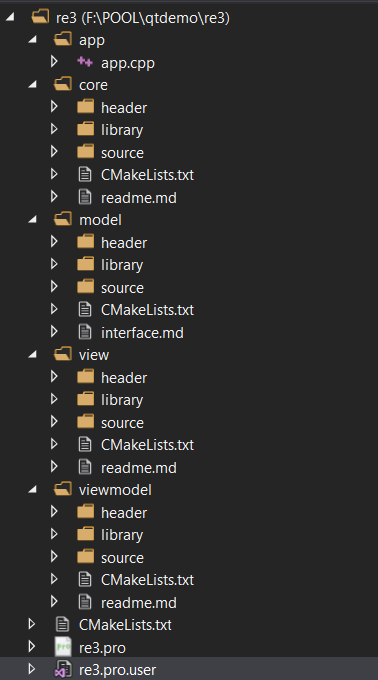
\includegraphics[width=0.3\textwidth]{image/codev2} 
\caption{系统原型.}
\end{center}
\end{figure}

运行界面如图8所示。 \\
\begin{figure}[h]
\begin{center}
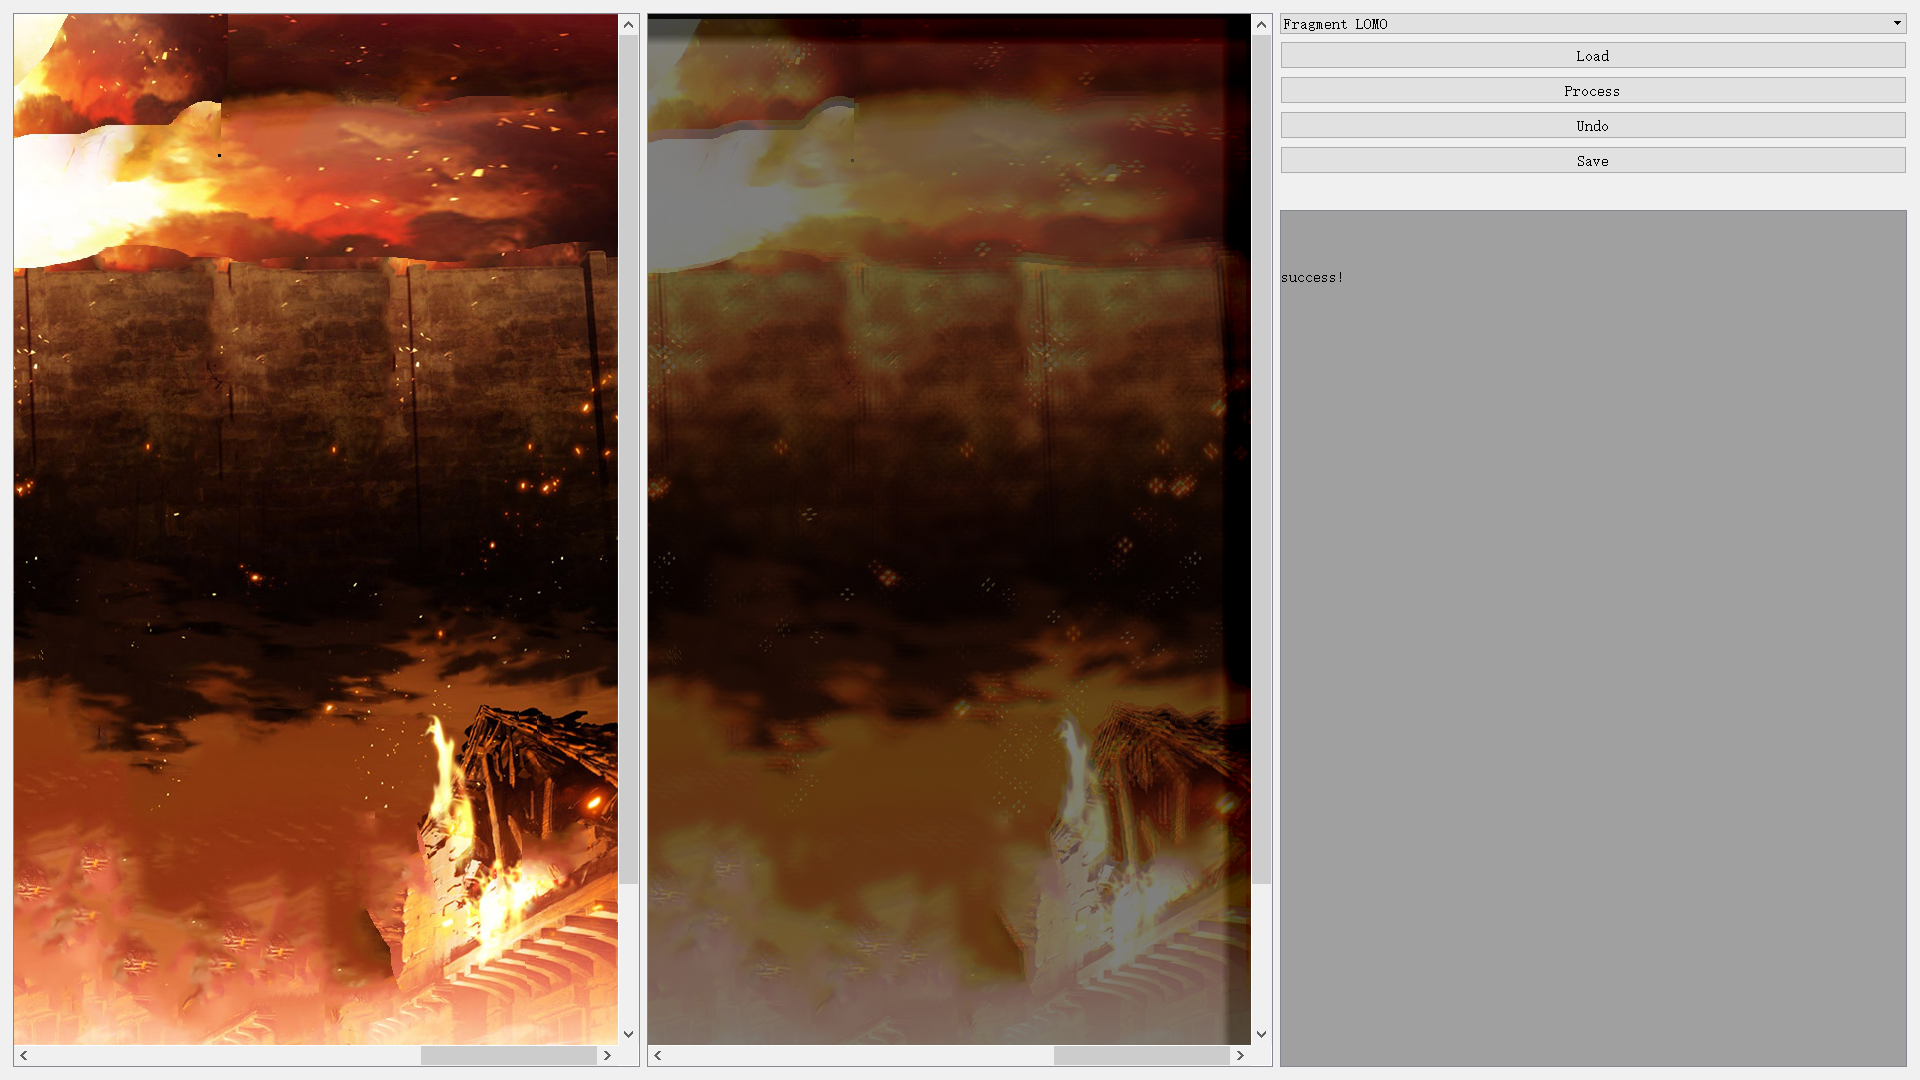
\includegraphics[width=0.9\textwidth]{image/second}
\caption{运行界面}
\end{center}
\end{figure}

\newpage
第二迭代的任务分配情况:\\\\
\begin{center}
\begin{tabular}{lr}
	图形界面开发  &林悦如 \\
	模型开发\\
	集成与测试	\\  
	算法层开发 &刘涵宇,林宇豪 \\
\end{tabular}
\end{center}

\paragraph*{第三轮迭代}
第三轮迭代中,我们继续完善系统的功能。将新的算法和GUI元素添加到软件中。\\
任务分配情况:\\\\
\begin{center}
\begin{tabular}{ll}
	项目文档,图形界面开发 &林宇豪\\  
	算法层开发 &刘涵宇\\
	系统集成	&林悦如	
\end{tabular}
\end{center}

\newpage
\section{软件截图}
\begin{figure}[h]
\begin{center}
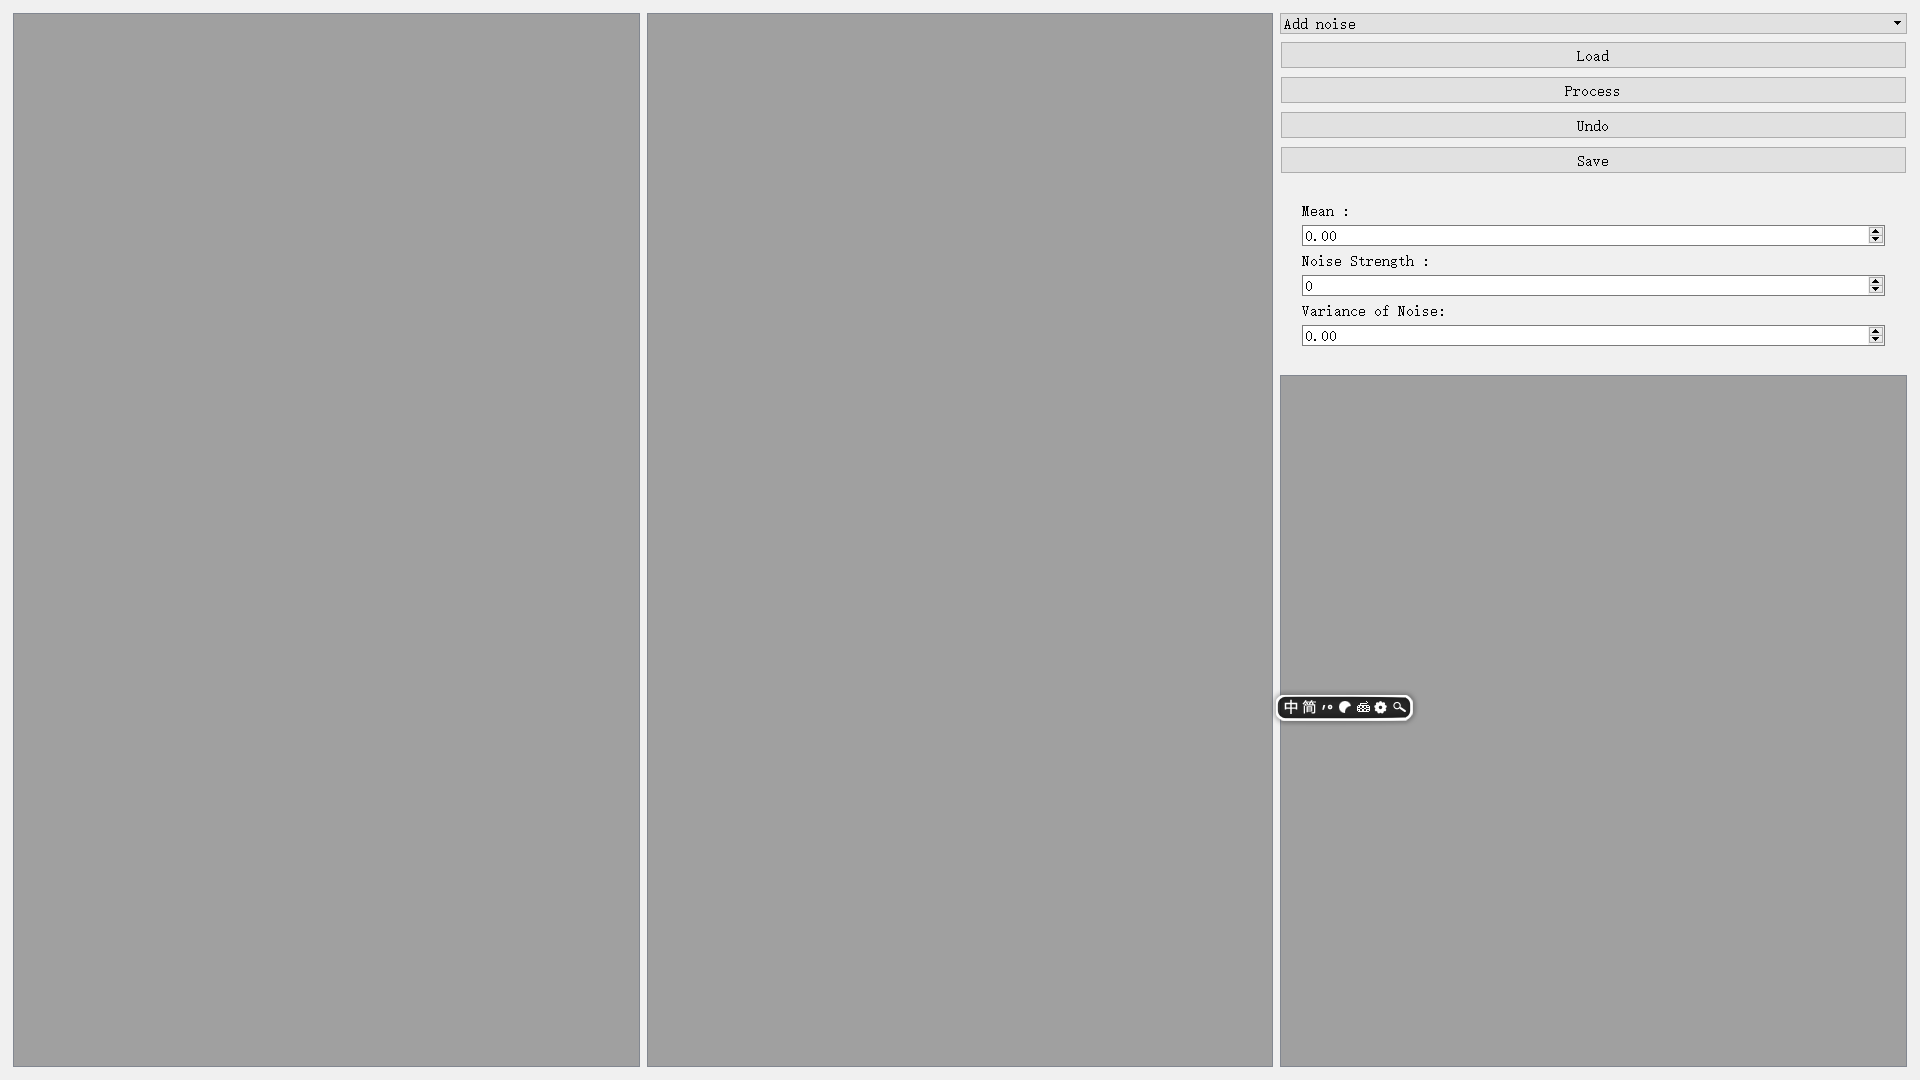
\includegraphics[width=\textwidth]{image/1} 
\caption{运行界面 1.}
\end{center}
\end{figure}

\begin{figure}[h]
\begin{center}
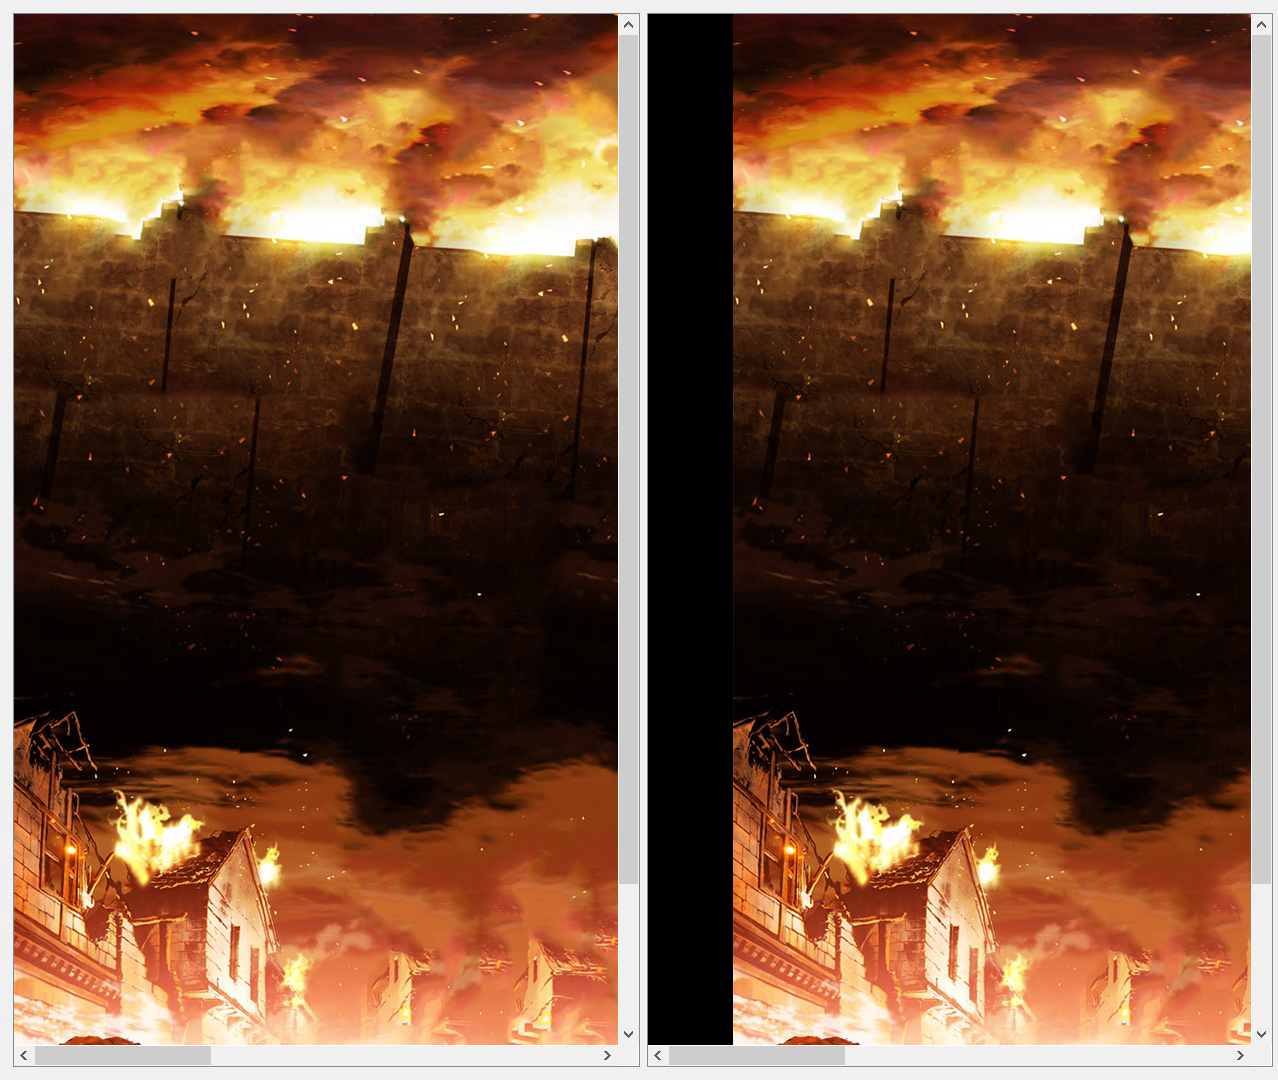
\includegraphics[width=\textwidth]{image/2} 
\caption{运行界面 2.}
\end{center}
\end{figure}

\begin{figure}[h]
\begin{center}
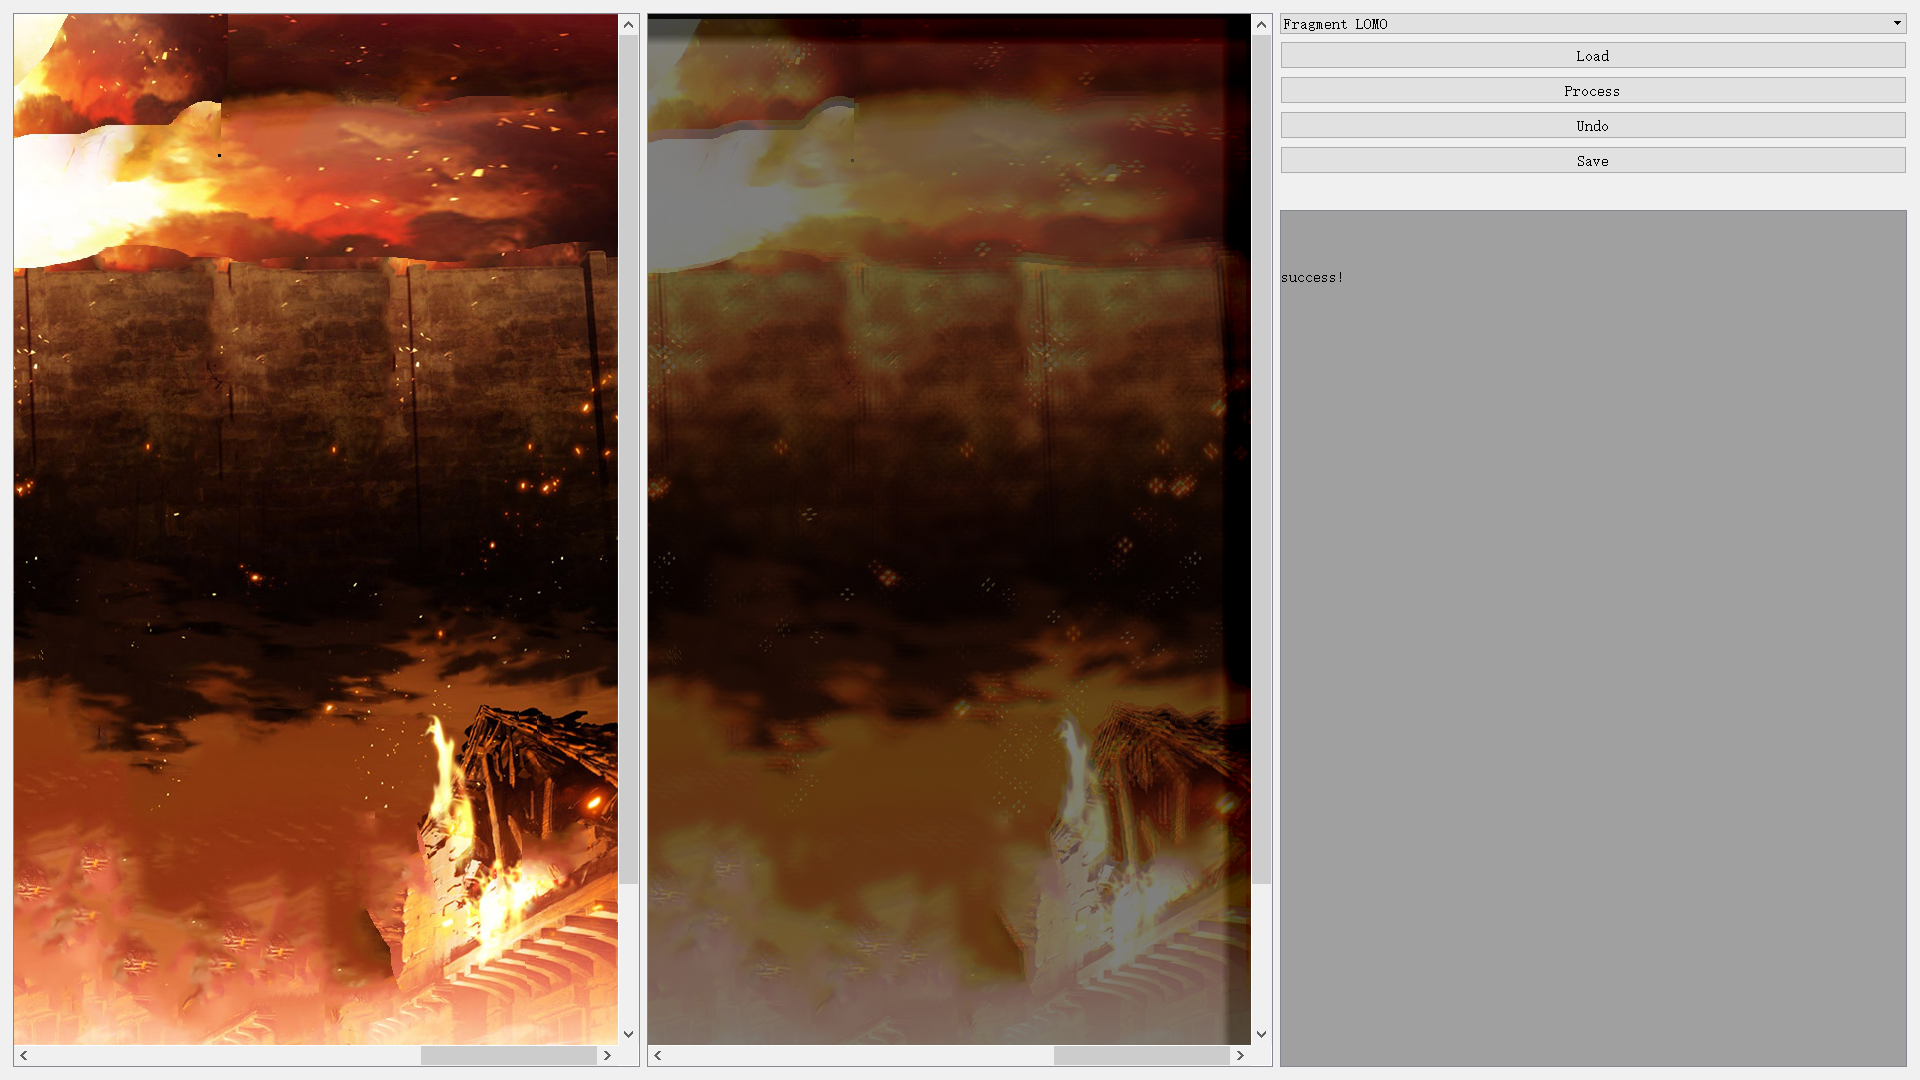
\includegraphics[width=\textwidth]{image/3} 
\caption{运行界面 3.}
\end{center}
\end{figure}

\begin{figure}[h]
\begin{center}
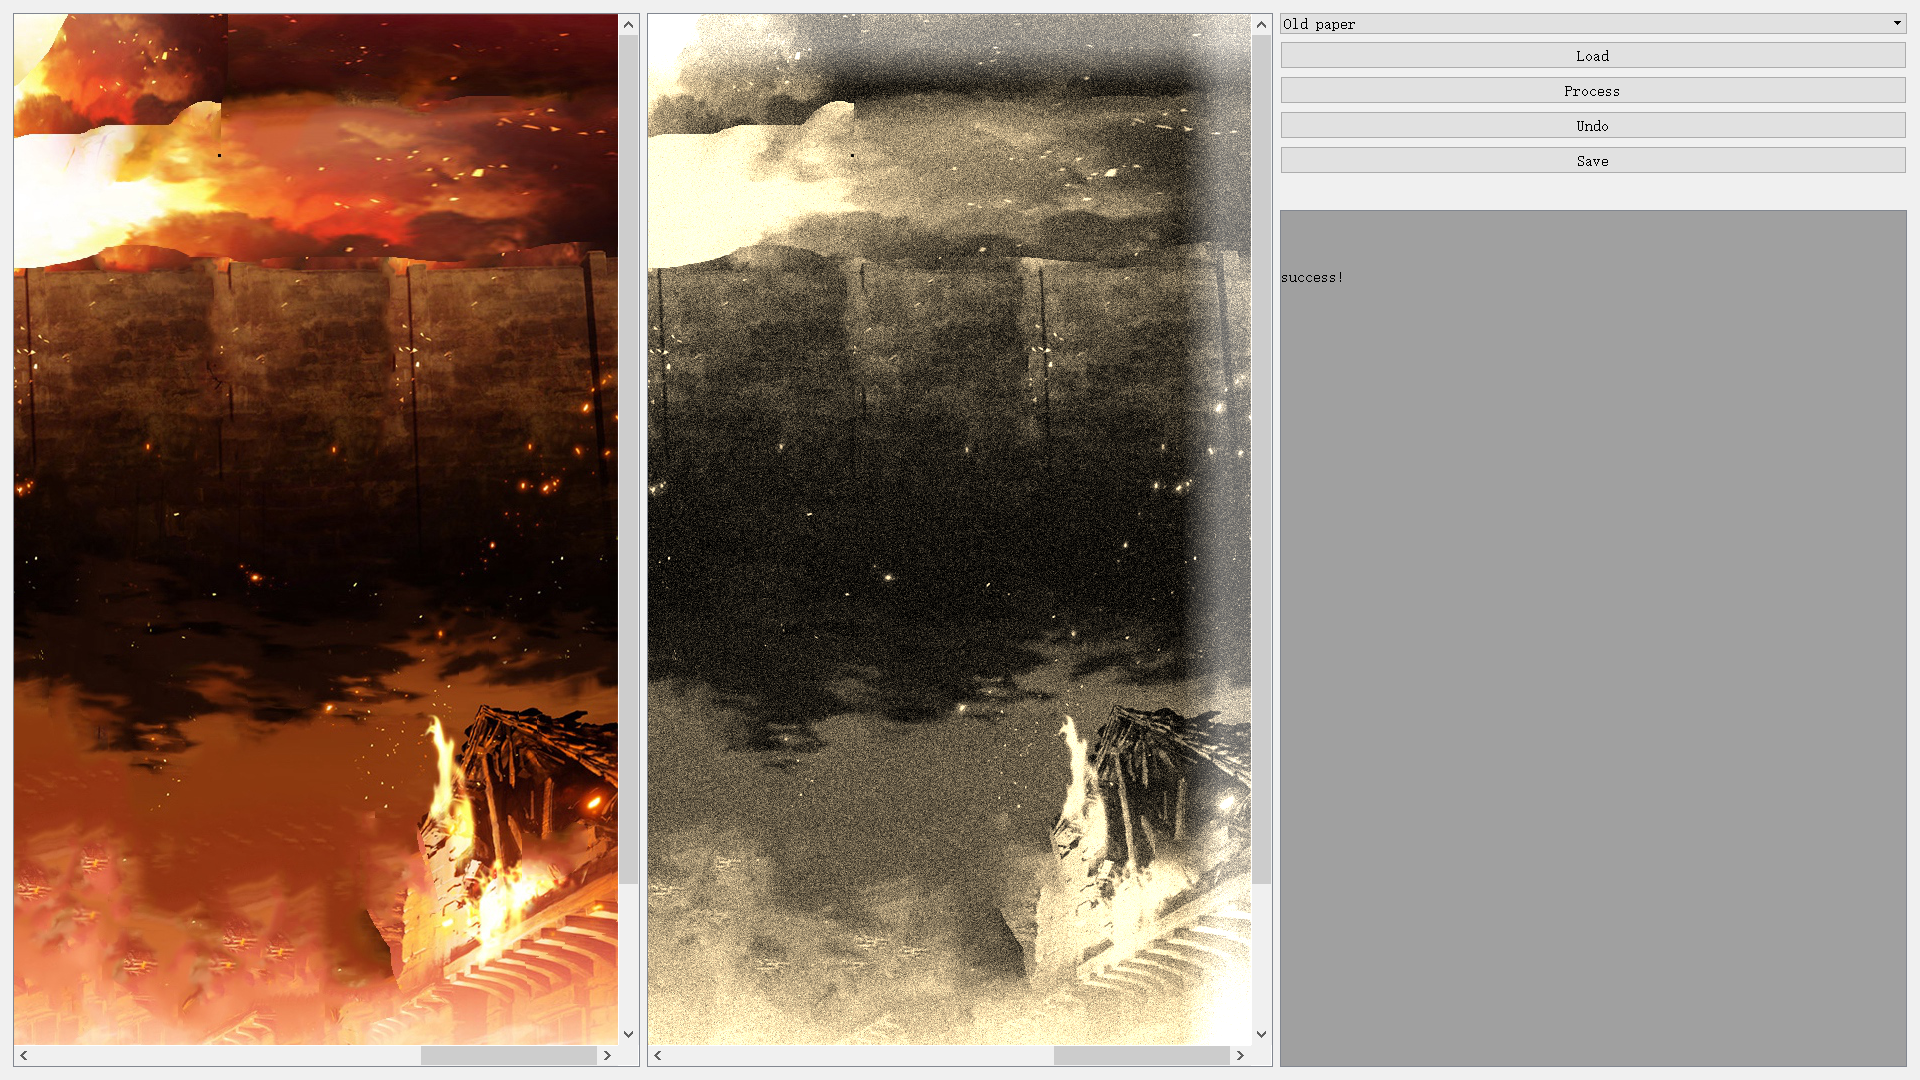
\includegraphics[width=\textwidth]{image/4} 
\caption{运行界面 4.}
\end{center}
\end{figure}

\subsection*{}
\newpage %this one is necessary 
\end{CJK}
\end{document}

